\begin{frame}
	\frametitle{$C_{3}$: Scalable Ontology-based Concept Detection}
	 {\small
	\begin{itemize}
 	  \item $C_{3}$ : A Scalable Semantic \alert{Hierarchical} Framework.
 	  \end{itemize}
	}
	\begin{center}\hspace*{-1cm} 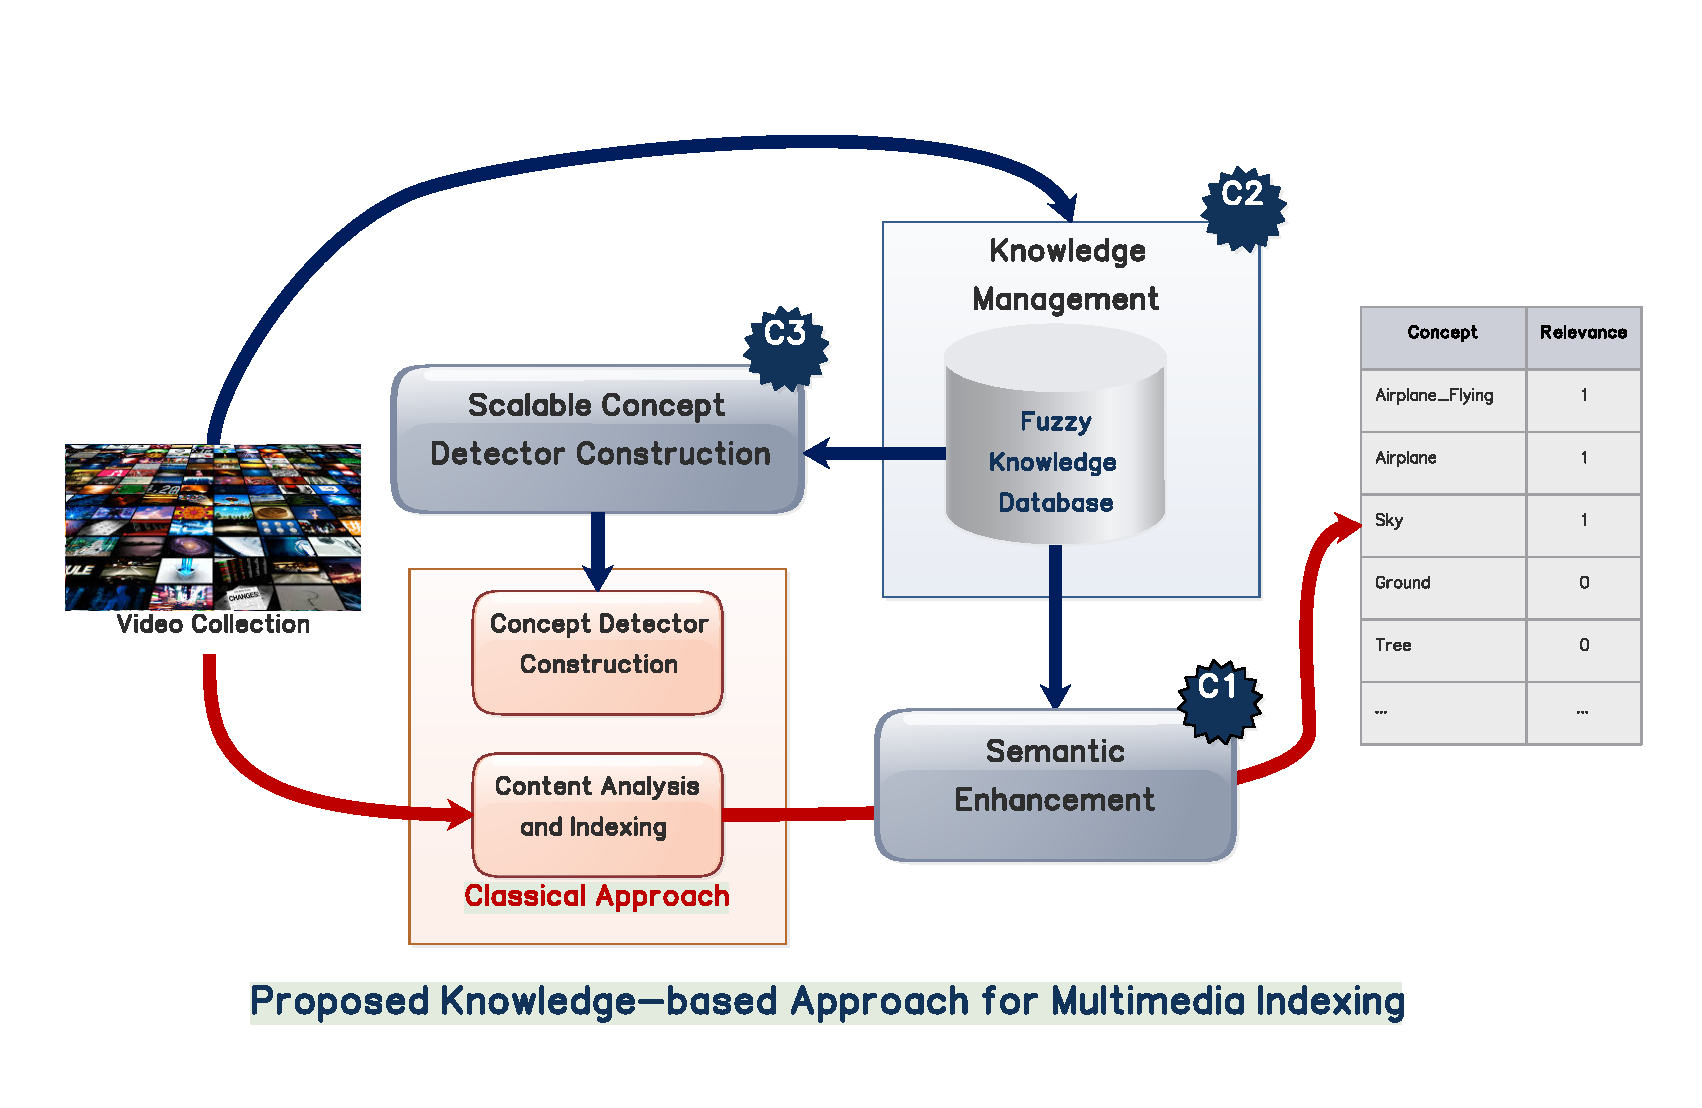
\includegraphics[scale=0.30]{graphics/contribution/contrib_overview_4} \end{center}

\end{frame}


\begin{frame}
	\frametitle{Classical Approach}
	\begin{block}{}
	 \begin{itemize}
	  \item Construct a \alert{dedicated} detector for each concept,
	  \item For a given content, all the detectors are fired.
	 \end{itemize}
	\end{block}
	\hspace*{-1cm}\centering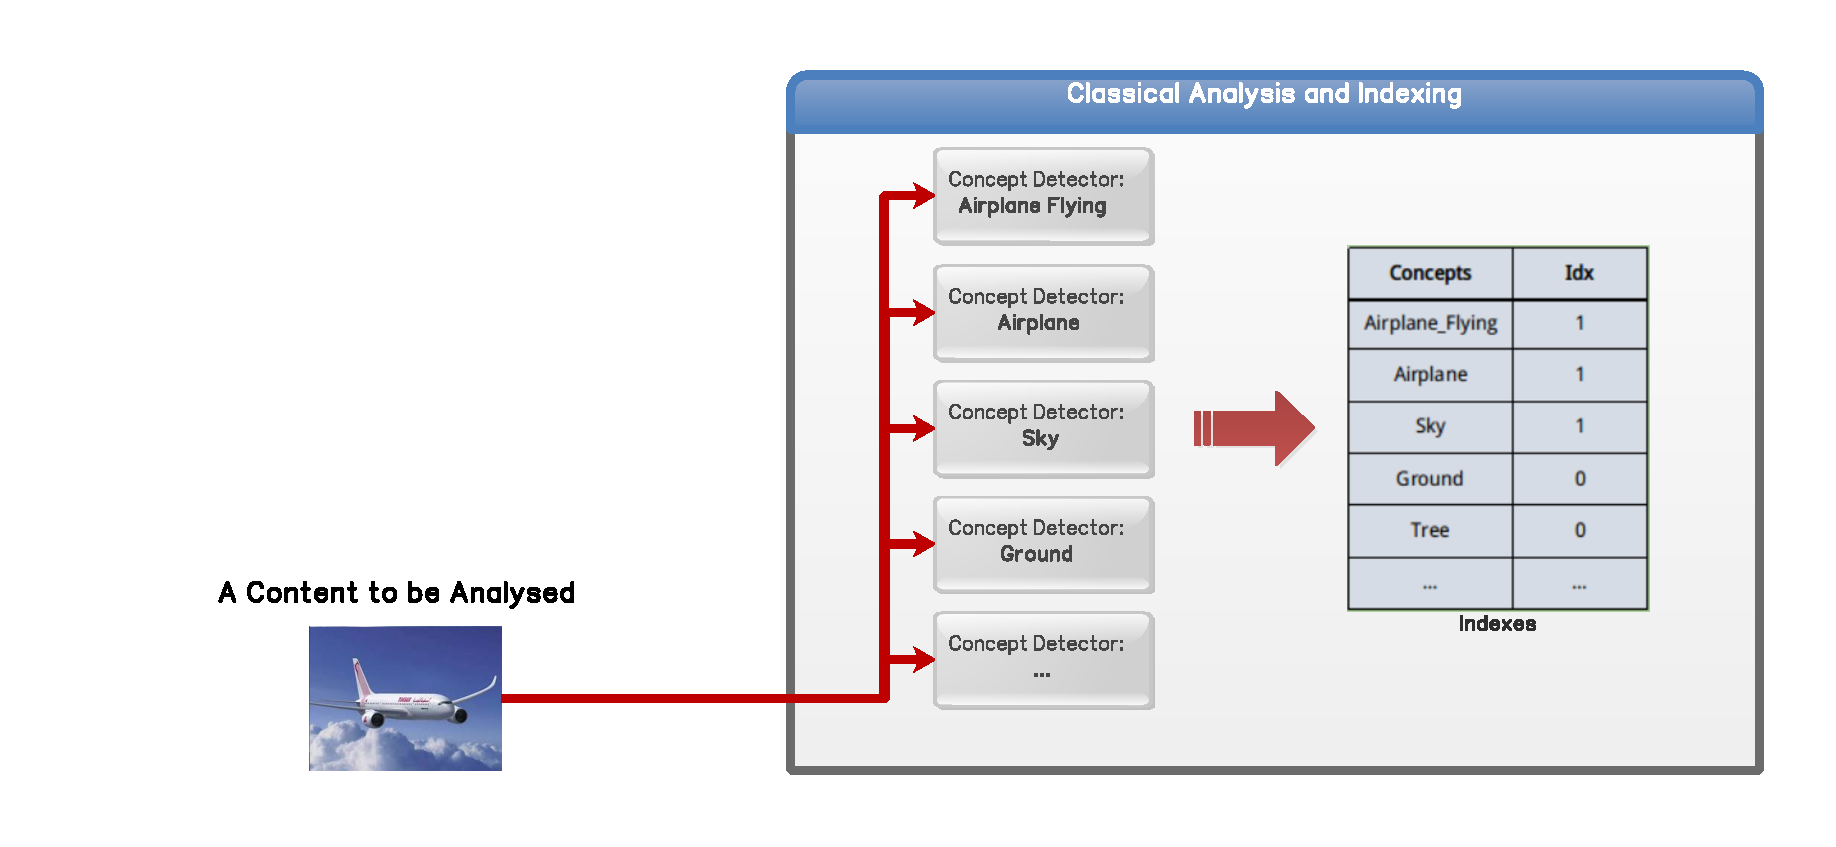
\includegraphics[scale=0.39]{graphics/c3/main_c3_1}
% 	\only<2>{\hspace*{-1cm}\centering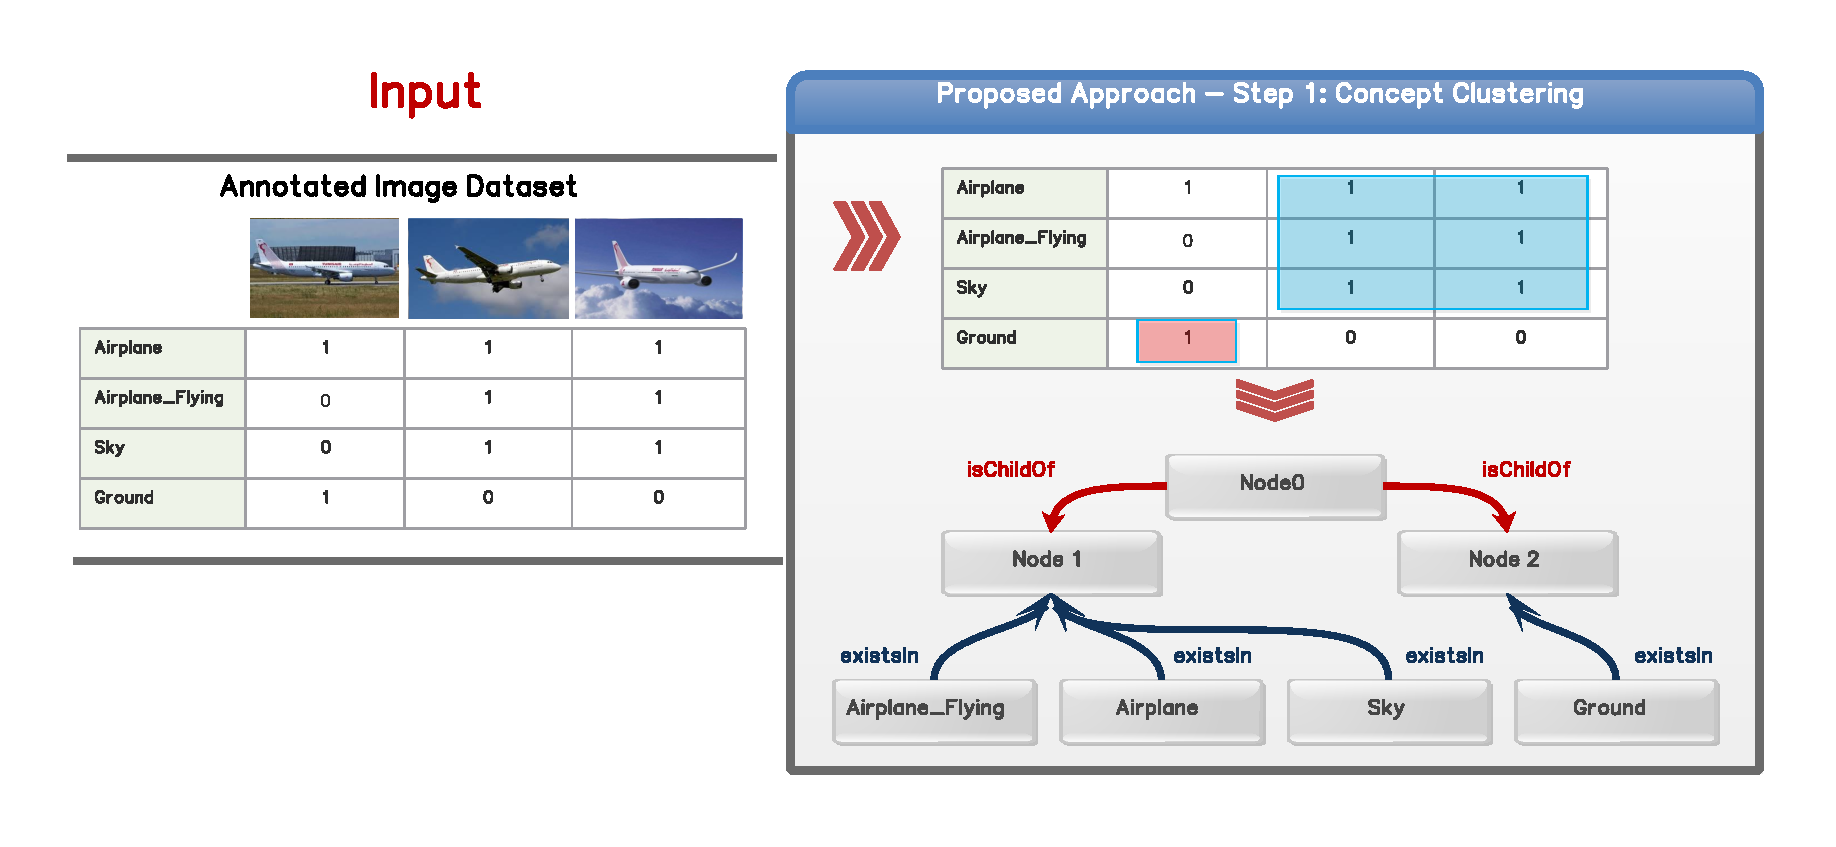
\includegraphics[scale=0.41]{graphics/c3/main_c3_2}}
% 	\only<3>{\hspace*{-1cm}\centering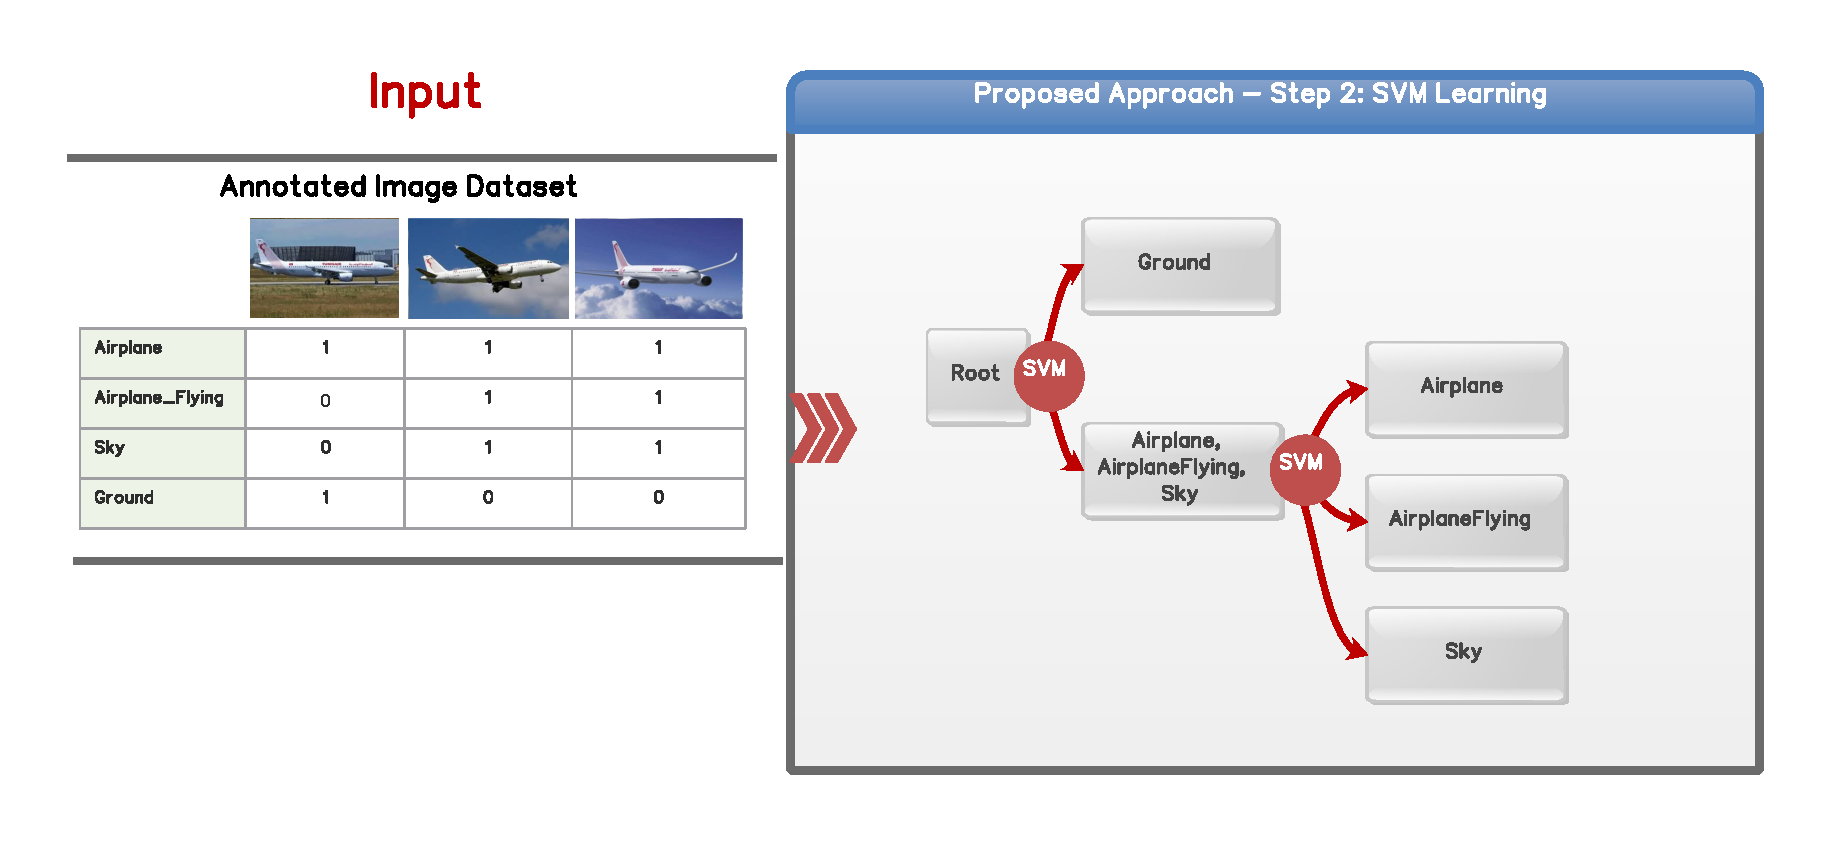
\includegraphics[scale=0.41]{graphics/c3/main_c3_3}}
% 	\only<4>{\hspace*{-1cm}\centering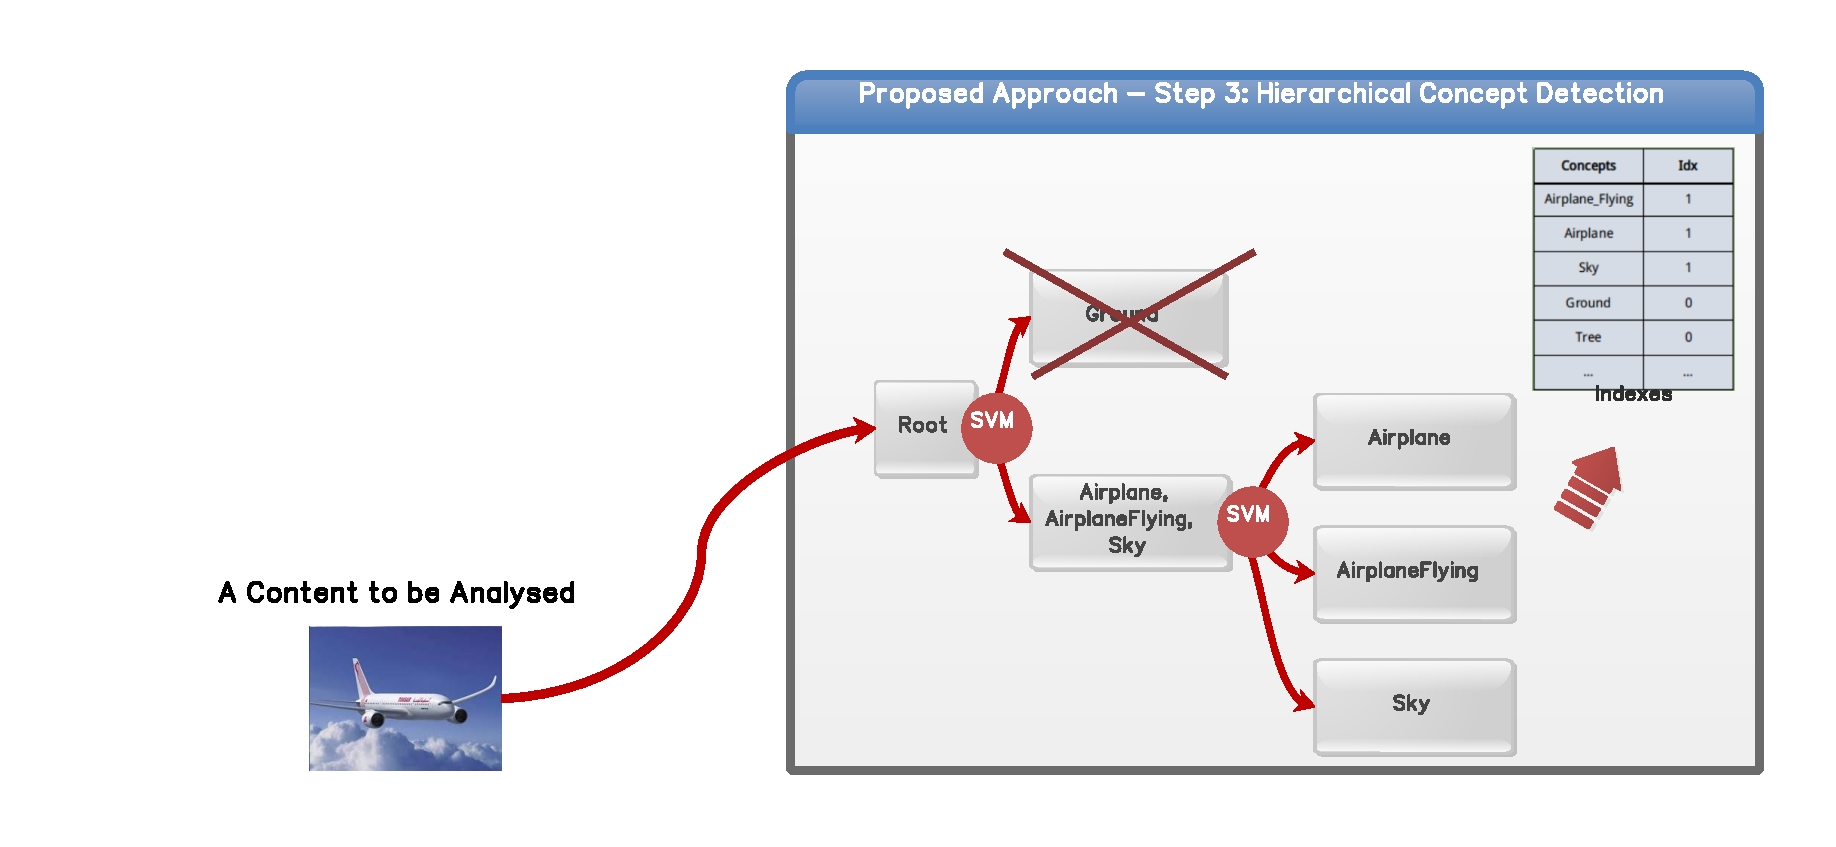
\includegraphics[scale=0.41]{graphics/c3/main_c3_4}}
\end{frame}

\begin{frame}
	\frametitle{$C_{3}$: Proposed Approach - Hierarchical Ontology Structure}
	\begin{block}{}
	 \begin{itemize}
	  \item An ontology structure based on concept \alert{hierarchy}, 
	  \item Two main roles: \textbf{isChildOf} and \textbf{existsIn}.
	 \end{itemize}
	\end{block}
	\hspace*{-1cm}\centering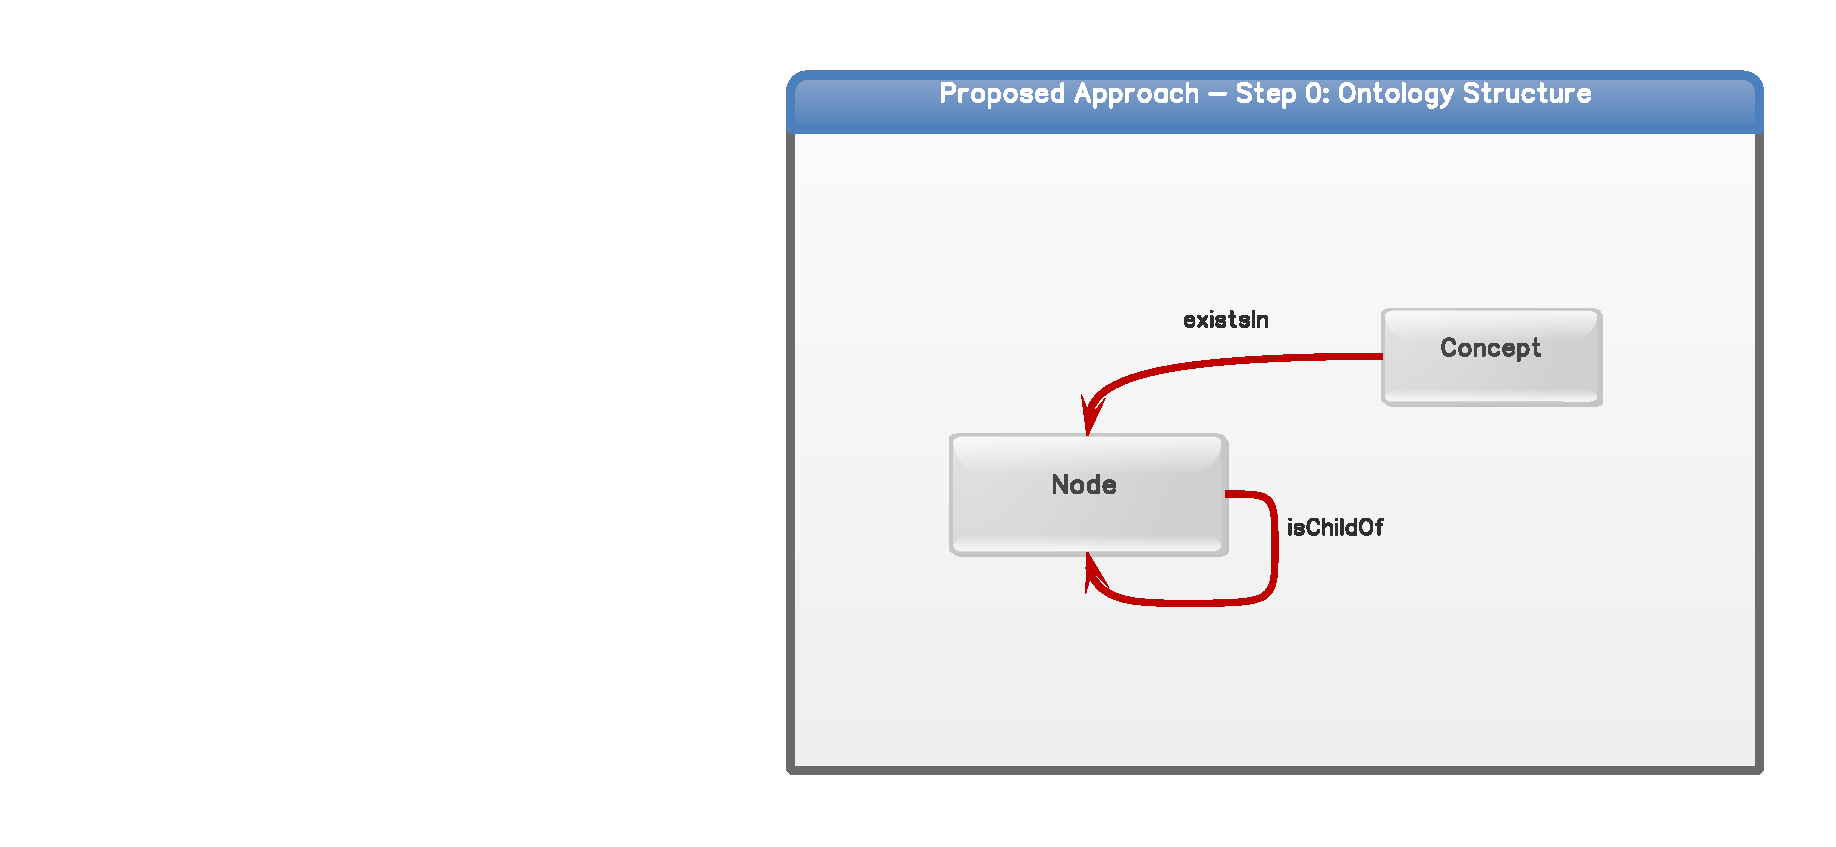
\includegraphics[scale=0.39]{graphics/c3/main_c3_0}
\end{frame}

\begin{frame}
	\frametitle{$C_{3}$: Proposed Approach - Knowledge Extraction}
	\begin{block}{}
	 \begin{itemize}
	  \item Clustering concept vectors using \alert{k-means},
	  \item Clustered conceps are populated within the ontology.
	 \end{itemize}
	\end{block}
	\hspace*{-1cm}\centering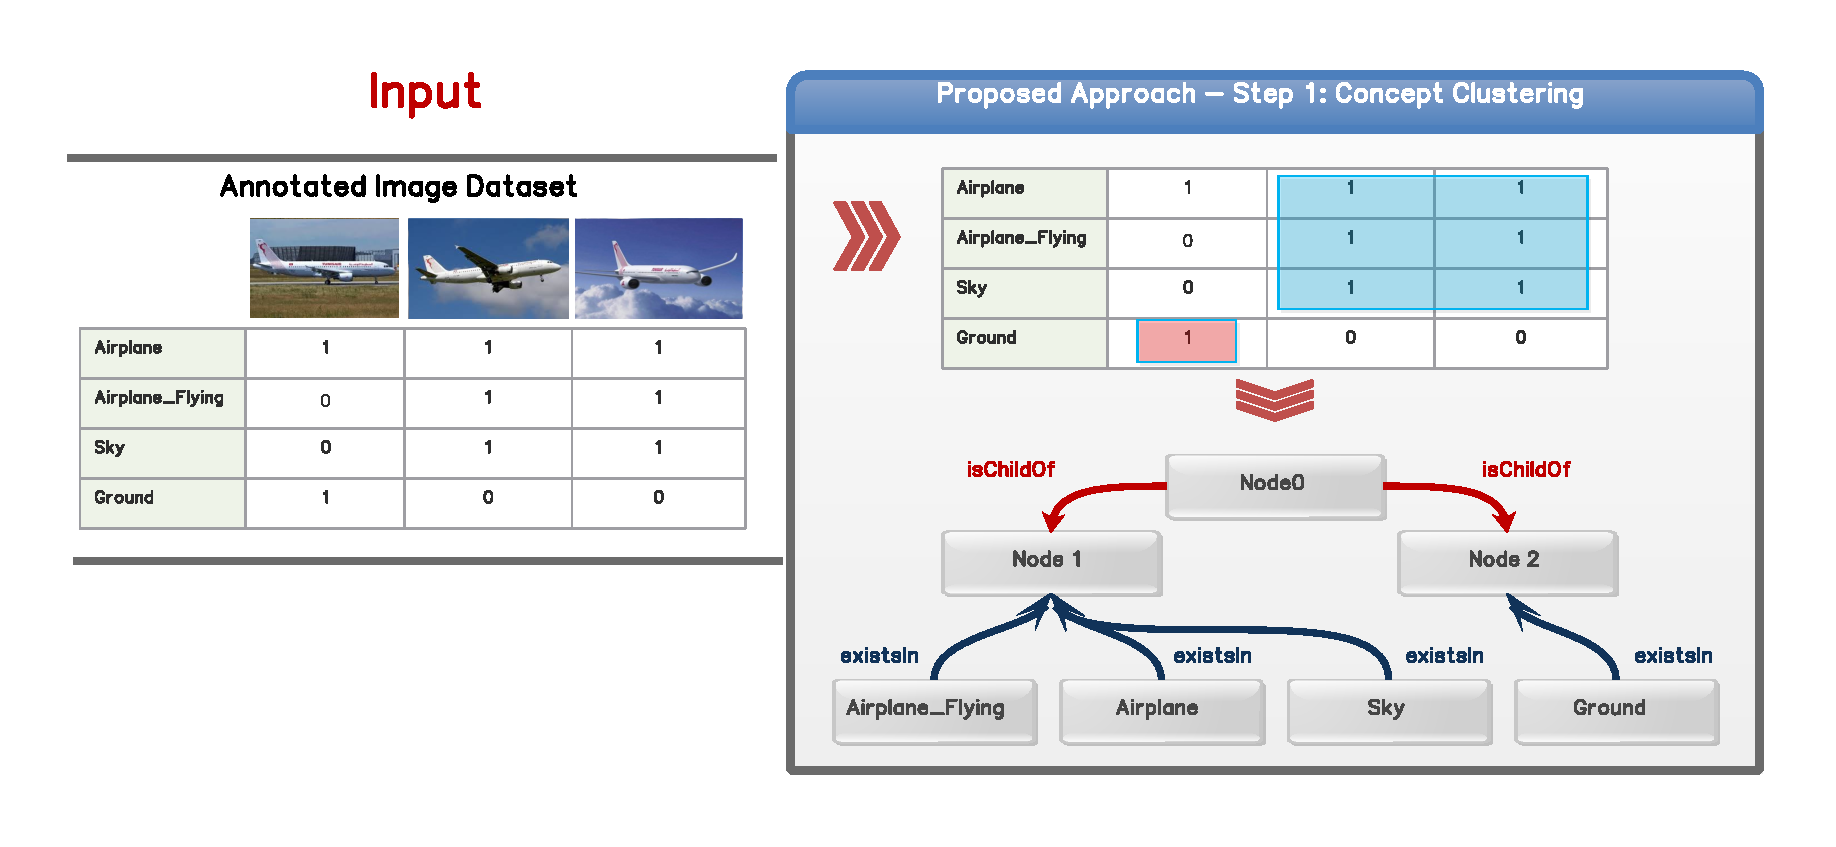
\includegraphics[scale=0.39]{graphics/c3/main_c3_2}
\end{frame}


\begin{frame}
	\frametitle{$C_{3}$: Hierarchical Semantic Detectors Construction}
	\begin{block}{}
	 \begin{itemize}
	  \item Extract \alert{\textsc{Sruf}} features from annotated images,
	  \item one-vs.-one linear kernel \alert{\textsc{Svm}} based learning algorithm.
	 \end{itemize}
	\end{block}
	\hspace*{-1cm}\centering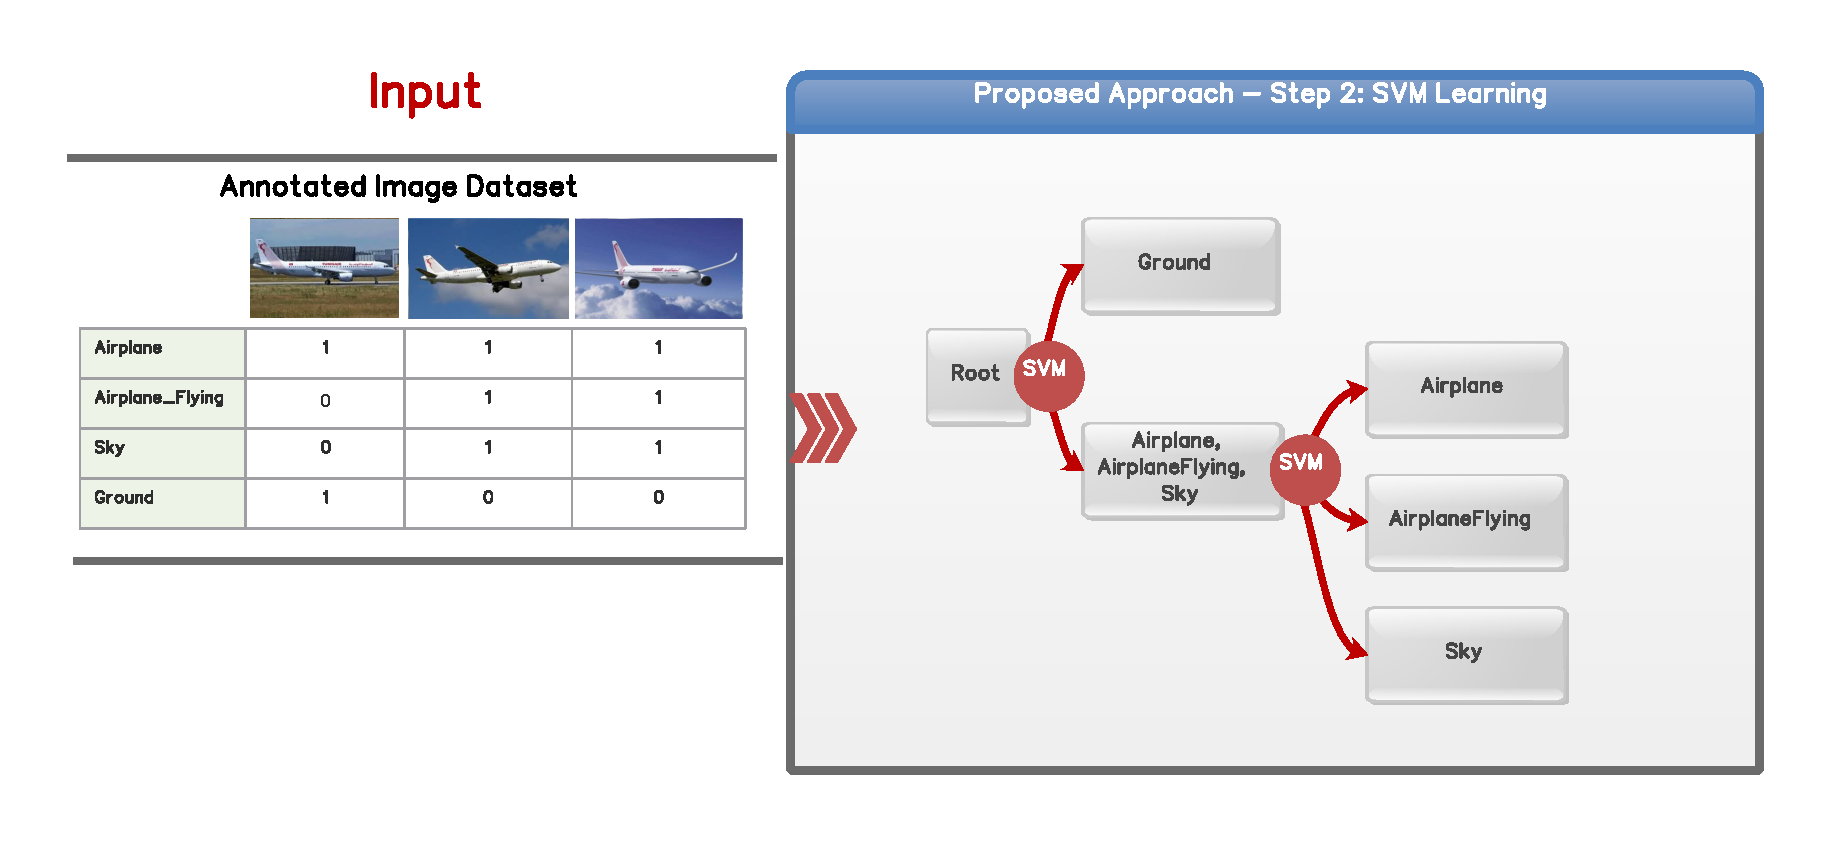
\includegraphics[scale=0.39]{graphics/c3/main_c3_3}
\end{frame}

\begin{frame}
	\frametitle{$C_{3}$: Hierarchical Semantic Image Annotation}
	\begin{block}{}
	 \begin{itemize}
	  \item \alert{Walking} the concepts hierarchy,
	  \item In each level, the \textsc{Svm} detects concepts to be \alert{excluded}.
	 \end{itemize}
	\end{block}
	\hspace*{-1cm}\centering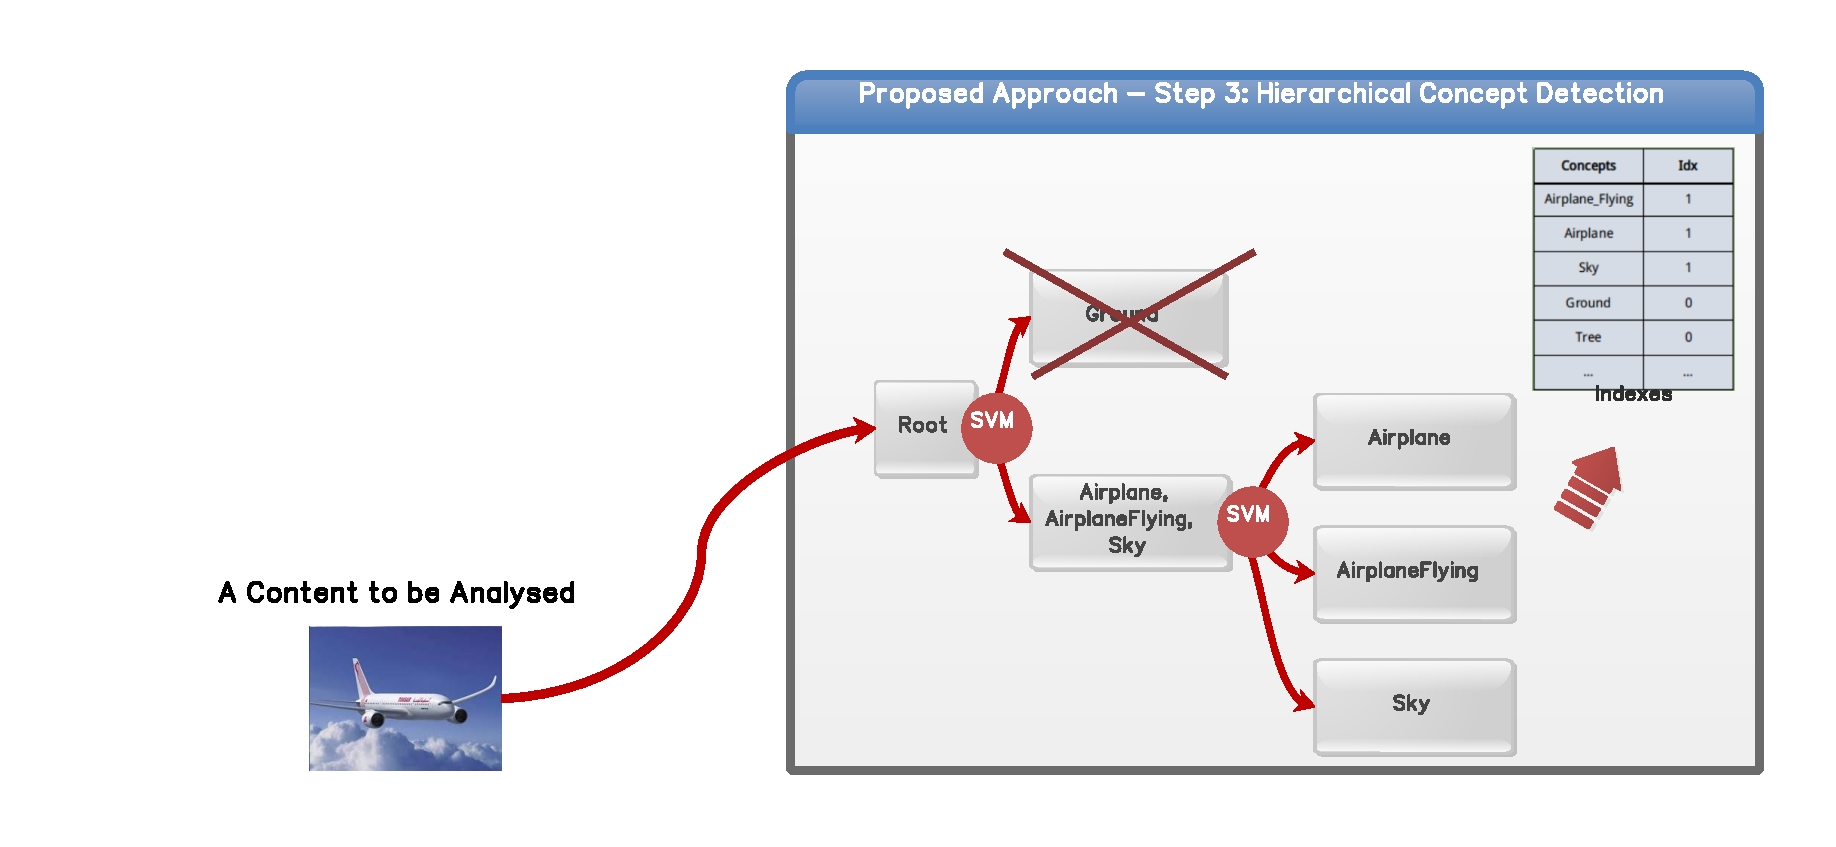
\includegraphics[scale=0.39]{graphics/c3/main_c3_4}
\end{frame}

\begin{frame}
	\frametitle{$C_{2}$: Experiments - Setup}
	\begin{exampleblock}{Experimentation Setup}
		{\small
		\begin{itemize}		
			\item \textsc{ImageClef 2015}
			\item Photo dataset : \alert{\textbf{500.000}} images \\ (only \textbf{1.500} images were annotated)
			\item \alert{251} semantic concepts
		\end{itemize}
		}
	\end{exampleblock}
\end{frame}

\begin{frame}
	\frametitle{$C_{2}$: Experiments - Results}
	\begin{exampleblock}{Accuracy Evaluation}
		{\small
		\begin{itemize}		
			\item Only \alert{$300.000$} images were annotated.
		\end{itemize}
		%\begin{table}
		\centering
		\begin{tabular}{ l| l l }
				\hline
				\textbf{\small } 	& \textbf{\small MAP} &	 \\
				\hline \hline
				\textbf{\small Best run}  & {\small $0,659507$}		& {\small(/SMIVA/21.run)} \\
				\textbf{\small Worst run} & {\small $0,000231898$}	&  \\
				\textbf{\small Average}	  & {\small $0,18673$} 		&  \\
				\textbf{\small Our best run~~}& {\small$0,0161687$} 	&  {\small(position $75/89$)} \\
				\hline
				\end{tabular}
		%\end{table}		

		}
	\end{exampleblock}
	%\pause
	\begin{exampleblock}{Scalability Evaluation}
		{\small
		\begin{itemize}		
			\item An average \alert{$52$} \textsc{Svm} classifiers were fired ($min=6$ and $max=175$) 
				instead of firing all the \alert{$251$} \textsc{Svm} classifiers
			\item \alert{Reducing about $80\%$ the number of concept to be detected}
		\end{itemize}
		}
	\end{exampleblock}
\end{frame}

\begin{frame}
	\frametitle{$C_{3}$: Related publication}
	\begin{block}{}
		\begin{itemize}
			\item \citep{Zarka2015a} \textbf{Zarka, M.}, Ben Ammar, A., \&{} Alimi, A. (2015). 
				Regimvid at imageclef 2015 scalable concept image annotation 
				task: Ontology based hierarchical image annotation. 
				In \emph{Working notes for CLEF 2015 conference , 
				Toulouse, France, September 8--11, 2015.}
		\end{itemize}
	\end{block}	
\end{frame}
